This section shows the characterization of no-clad BCF-12 fibers from Saint-Gobain, which are the fibers used in the TRITIUM experiment. These measurements are compared to other measurements that was made using single clad and multiclad BCF-12 fibers to quantify how the clad affect to several parameters of scintillating fibers.

It is an interesting comparison because, although commercial clads cannot be used for the TRITIUM experiment, they can be developed with a low enough thickness. For example, clads with a thickness of the order of tens of nanometers can be achieved by electrodeposition techniques.

As it was shown in section \ref{subsec:PlasticScintillators}, the difference between these three types of fibers is that no clad fibers only consist of a polystyrene core with a refractive index of $1.60$ whereas, in single clad fibers, the polystyrene core has an acrylic cover (PMMA) with a thickness of $30~\mu\meter$ and a refractive index of $1.49$ and, in multiclad fibers, this acrylic cover has another fluor-acrylic cover with a thickness of $10~\mu\meter$ and a refractive index of 1.42.

%The first measurement that was made is the measurement of the diameter of the fiber. It is important because scintillating molecules are only present in the polystyrene core and we need to know whether the entire polystyrene core is the same size or not. Three different samples of each type of fiber were measured and the results are presented in Table \ ref {}.

%TABLAAA DIAMETROOOS

%Therefore, we can see that all fibers have the same external size, which means that the diameter of the polystyrene core is smaller for single clad fibers ($0.97~\mm$) and even smaller for multiclad fibers ($0.96~\mm$). It is an important result since...

This characterization was performed at the level of a single scintillating fiber and the parameters measured for every fiber type are the fiber collection efficiency and the uncertainty in the fiber response due to the conditioning process developed in TRITIUM. The reference measure that will be used for that is the number of photons per second that reach the active area of the photosensor.
%r8520-406

To measure this parameter, a calibrated PMT, model R8520-06SEL, was used, whose quantum efficiency at the working wavelength, $29.76\%$, measured by the provider, Hamamatsu. To measure this parameter, the PCB described in section \ref{subsubsec:PMTsElectronicalSystem} is needed to work without the internal gain of the PMT and the Keithley 6487 Picoammeter/Voltage Source is used to measure the output current of the PMTs. The number of photons per second can be known from the Keithley measurement using the equation \ref{eq:NumPhotonsFromIntensityPMT} with $QE=0.2976$ and $CE=1$. A simplified scheme of the set up used for this characterization is shown in Figure \ref{fig:SetUpFiberCharacterization}.

\begin{figure}[h]
\centering
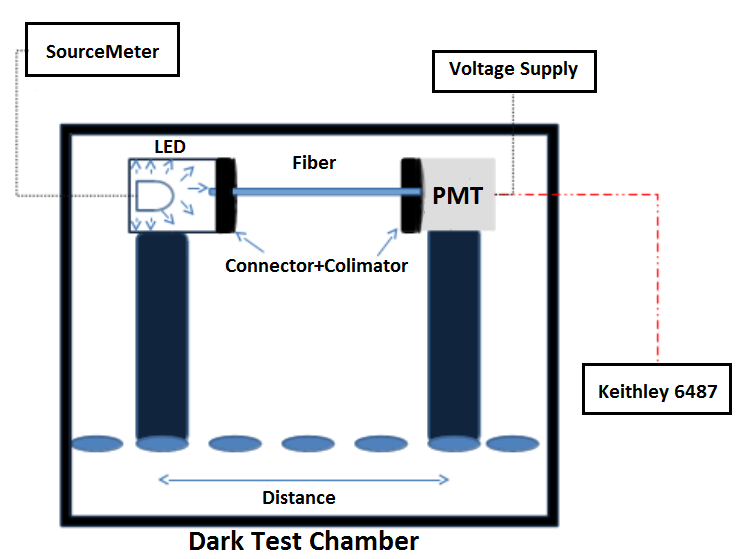
\includegraphics[scale=0.6]{4ResearchAndDevelopments/41Fibers/SetUp_Fiber_Characterization.png}
\caption{Set up used for fiber characterization.\label{fig:SetUpFiberCharacterization}}
\end{figure}

It consists of an optical structure in which a LED and a PMT are fixed to the specific distance between them, established by the user. The LED, model LED435-03 from the Roithner LaserTechnik Gmbh company \cite{LEDRLT}, is used to reproduce the light emission by the fibers used. The emission spectrum of the LED is shown in Figure \ref{fig:LEDSpectrumTritium}, which was experimentaly measured using a spectrometer and fitted to a Gaussian function. The emission peak of this LED is produced at $433.9~\nano\meter$ with a FWHM of $18.4~\nm$. 

\begin{figure}[h]
\centering
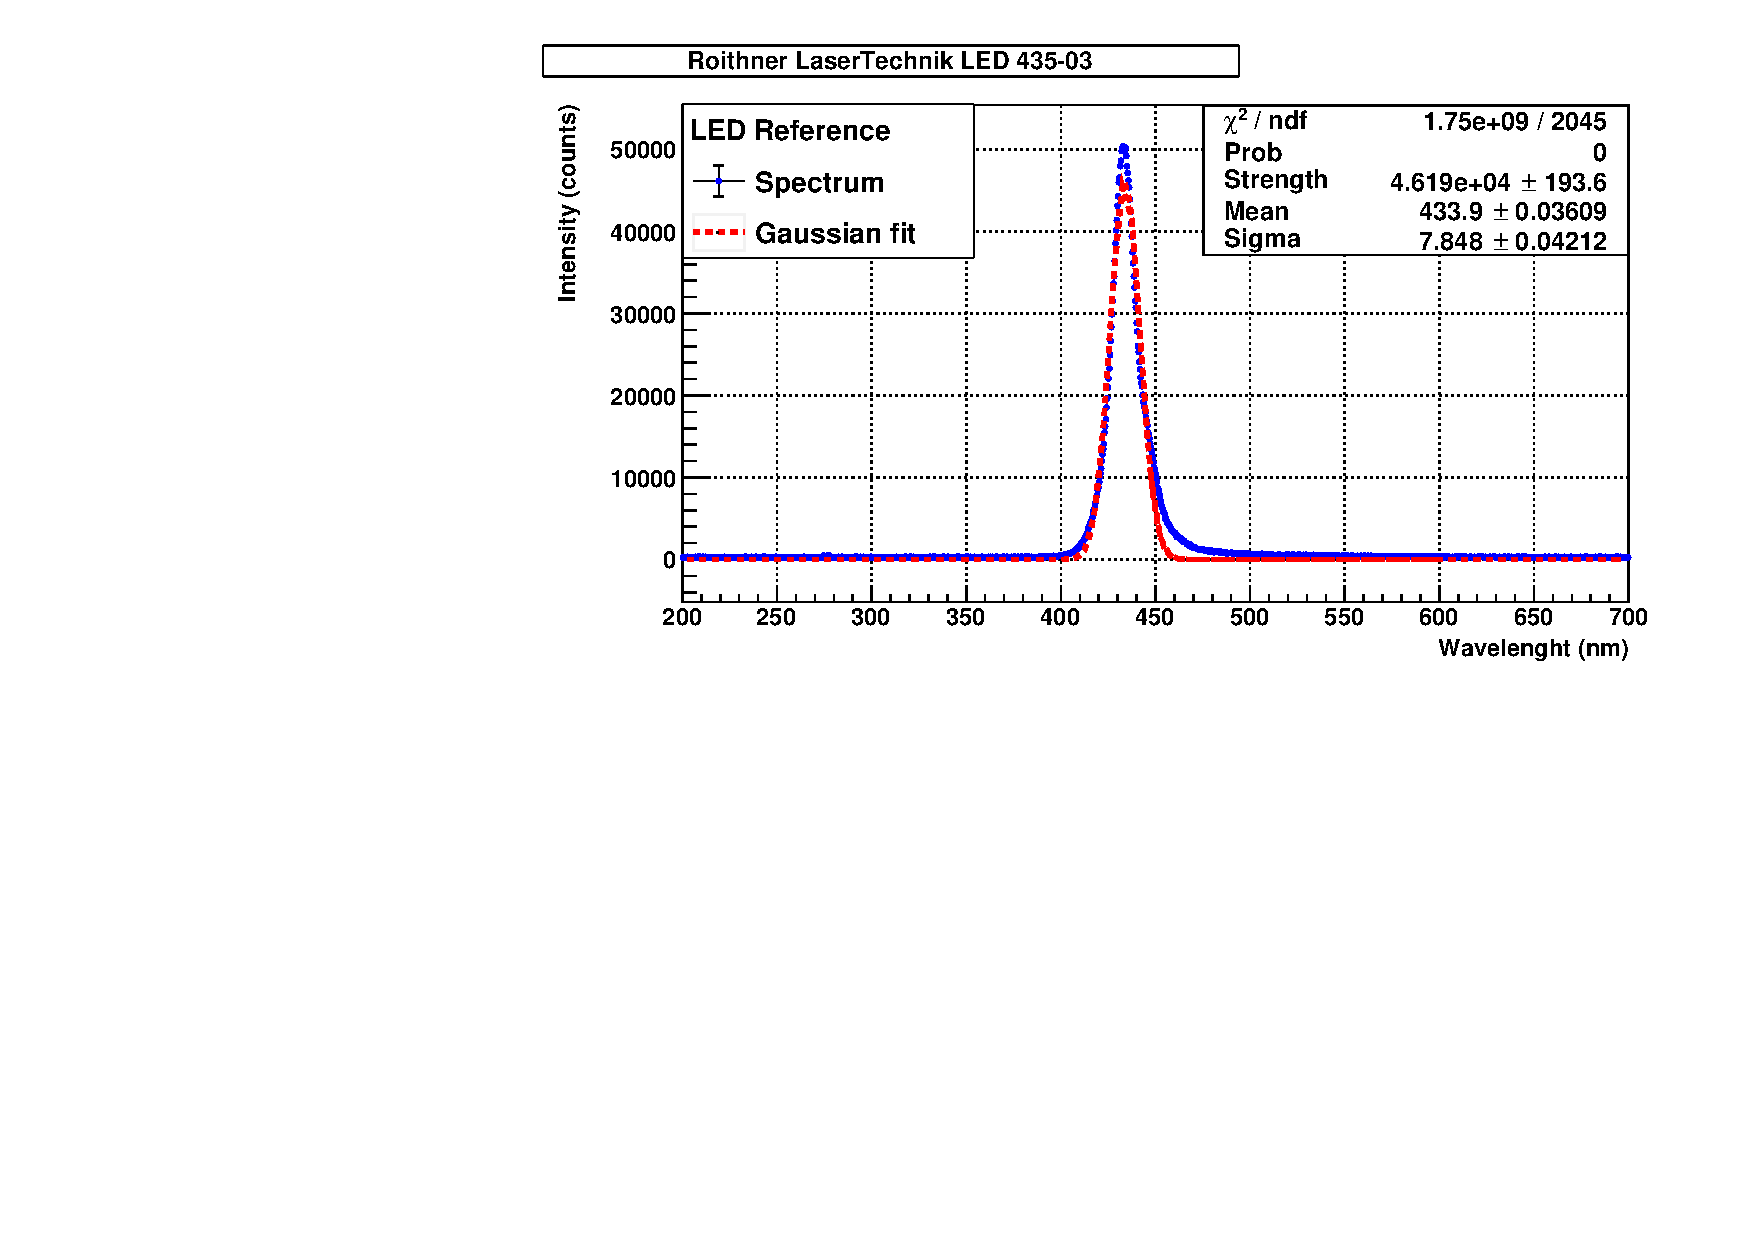
\includegraphics[scale=0.6]{4ResearchAndDevelopments/41Fibers/LED_TRITIUM.pdf}
\caption{Emission spectrum measured for the LED model 435-03 from Roithner LaserTechnik Gmbh Company.\label{fig:LEDSpectrumTritium}}
\end{figure}

The fiber will be fixed between the LED and the PMT, whose distance is configured based on the length of the fiber, $20~\cm$ for this study, and optic grease \cite{OpticalGrease} was used for optimal optical coupling between the fiber and the PMT. Two collimators are used to ensure that the photons detected in the PMT are only those that come from the LED and travel through the fiber and two connectors, type FH-ST\footnote{FH-ST is a quick assembly connector for $1~\mm$ POF} from RoHS company \cite{}, were placed to the ends of the fiber and used to fix it to the system. 